\chapter{Introduction}

Traffic lights constitute the primary mechanism for regulating vehicular flow at urban intersections, and their correct interpretation is indispensable for road safety. As Advanced Driver Assistance Systems (ADAS) and fully autonomous vehicles become increasingly prevalent, the ability to detect and classify traffic light states reliably and in real time represents a fundamental requirement of any visual perception pipeline. This project addresses the challenge of detecting three traffic light states — go, stop, and warning — from dashcam video footage using a deep learning approach based on the You Only Look Once version 8 (YOLOv8) architecture.

\section{Background}

Traffic lights govern the movement of vehicles at approximately 50\% of urban intersections worldwide, making their accurate perception a safety-critical function for any automated driving system. ADAS platforms, which assist human drivers through functionalities such as automatic braking and intersection warnings, depend on visual perception modules that can identify traffic signal states under the full diversity of real-world driving conditions.

Traditional rule-based vision systems have been employed for this task in earlier works. Colour-threshold segmentation identifies candidate light regions by isolating pixels within a defined hue range in the HSV colour space. Haar cascade classifiers extend this by learning rectangular feature patterns from positive and negative training examples. However, both approaches exhibit significant performance degradation under illumination variation, partial occlusion, and variation in distance between the camera and the traffic light, as these systems encode fixed handcrafted representations that do not generalise beyond the specific conditions encountered during their design.

Deep learning, and particularly Convolutional Neural Networks (CNNs), has fundamentally transformed the field of object detection. CNN-based detectors learn hierarchical feature representations directly from annotated training data, enabling generalisation across a wide range of appearance variations. Among CNN-based detection frameworks, the You Only Look Once (YOLO) family of architectures has demonstrated exceptional performance in real-time detection scenarios due to its single-pass inference design, wherein both object localisation and classification are performed by a single forward pass of the network.

\section{Problem Statement}

The central task of this project is to detect traffic lights in dashcam video frames and classify their state into one of three semantic categories: go (green light), stop (red light), and warning (yellow or amber light). Three principal technical challenges are identified:

\begin{enumerate}
    \item \textbf{Small object size:} At typical driving distances, traffic lights occupy approximately 0.05\% of the total image area. This small spatial footprint places stringent demands on the detector's ability to resolve fine-grained features from low-resolution regions of the input image.
    \item \textbf{Class imbalance:} The warning class represents only approximately 2.8\% of annotated instances in the training data. Without correction, a model trained on this distribution would be biased toward the dominant stop and go classes, potentially failing to detect warning lights with sufficient reliability.
    \item \textbf{Sequential frame leakage:} The dataset consists of sequential video clips captured from a moving vehicle. Randomly partitioning frames across training and validation sets would place visually near-identical consecutive frames in both splits, causing an inflated validation accuracy that does not reflect the model's true generalisation capability on unseen sequences.
\end{enumerate}

\section{Objectives and Scope}

\subsection{Objectives}

\begin{itemize}
    \item To develop an end-to-end deep learning pipeline for traffic light state detection, achieving a mean Average Precision at 50\% Intersection over Union (mAP@50) above 0.70 on the validation set.
    \item To address class imbalance and small object detection through targeted preprocessing strategies, including sequence-aware data partitioning and oversampling of the underrepresented warning class.
    \item To evaluate the trained model on an unseen test split and export the final model weights to the Open Neural Network Exchange (ONNX) format for cross-platform deployment.
\end{itemize}

\subsection{Scope}

\begin{itemize}
    \item The dataset used is exclusively the LISA Traffic Light Dataset in Supervisely JSON annotation format.
    \item Detection is limited to three semantic classes: go, stop, and warning.
    \item The input domain is restricted to the dashcam perspective, specifically a forward-facing camera mounted at driver's-eye level.
    \item Model evaluation is conducted on the provided test split; no real-world video capture is performed as part of this project.
\end{itemize}

\section{Literature Review}

Early approaches to traffic light detection relied on classical computer vision techniques that operate on handcrafted features. Colour segmentation methods identify candidate light regions by thresholding pixels in the Hue-Saturation-Value (HSV) colour space within ranges corresponding to red, green, and yellow. These are frequently combined with morphological filtering and blob analysis to localise circular light fixtures. Haar cascade classifiers and Histogram of Oriented Gradients (HOG) descriptors combined with Support Vector Machine (SVM) classifiers extended this framework by learning from labelled examples. While effective under controlled laboratory conditions, such methods are inherently sensitive to illumination variation, lens flare, adverse weather, and partial occlusion, as the decision boundaries are fixed at design time and cannot adapt to unseen appearance distributions.

The introduction of CNN-based object detectors substantially improved detection accuracy under real-world conditions. The Region-based CNN (Faster R-CNN) framework proposed a two-stage detection paradigm: a Region Proposal Network (RPN) first generates candidate bounding box proposals, which are then classified and refined by a second sub-network. Single Shot MultiBox Detector (SSD) and RetinaNet achieved competitive accuracy in a single-stage design by predicting detections directly from dense anchor grids at multiple feature pyramid levels. RetinaNet introduced the Focal Loss function to address foreground-background class imbalance during training. While these models offered improved generalisation, the accuracy-versus-speed trade-off remained a challenge: two-stage detectors delivered high accuracy at the cost of inference latency incompatible with real-time requirements.

The YOLO family of detectors was introduced by Redmon et al.\ in 2016, proposing the first architecture to frame object detection as a single regression problem solved in one network forward pass, enabling real-time inference at over 45 frames per second. YOLOv3 extended this with a multi-scale Feature Pyramid Network (FPN) neck that combines feature maps from multiple backbone stages, improving detection of small objects. YOLOv8, released by Ultralytics in 2023, introduces Cross-Stage Partial bottleneck blocks with two convolutions (C2f) in the backbone, improving gradient flow and reducing parameter redundancy, alongside an anchor-free detection head that directly predicts box centre coordinates and dimensions without relying on predefined anchor sizes.

Transfer learning from large-scale datasets has been shown to be a highly effective strategy for traffic light detection. Initialising model weights from a checkpoint pre-trained on the Common Objects in Context (COCO) dataset endows the backbone with learned representations of general visual features — edges, textures, and colour gradients — that transfer readily to the traffic light detection domain. Prior works applying YOLO-family architectures with COCO-pretrained initialisation to traffic light detection have reported mAP@50 values in the range of 0.72 to 0.89 across various dataset benchmarks, confirming the suitability of this approach for the present task.

\section{Methodology}

The project follows a seven-stage pipeline: (1) dataset acquisition and format understanding, (2) exploratory data analysis, (3) label format conversion from Supervisely JSON to YOLO normalised text format, (4) sequence-aware data partitioning to prevent temporal leakage, (5) class imbalance correction through oversampling of warning-class sequences, (6) model training via transfer learning from COCO-pretrained YOLOv8s weights, and (7) model evaluation on the unseen test set and export to ONNX format for deployment. The overall system pipeline is illustrated in Figure~\ref{fig:pipeline}.

\begin{figure}[p]
    \begin{center}
        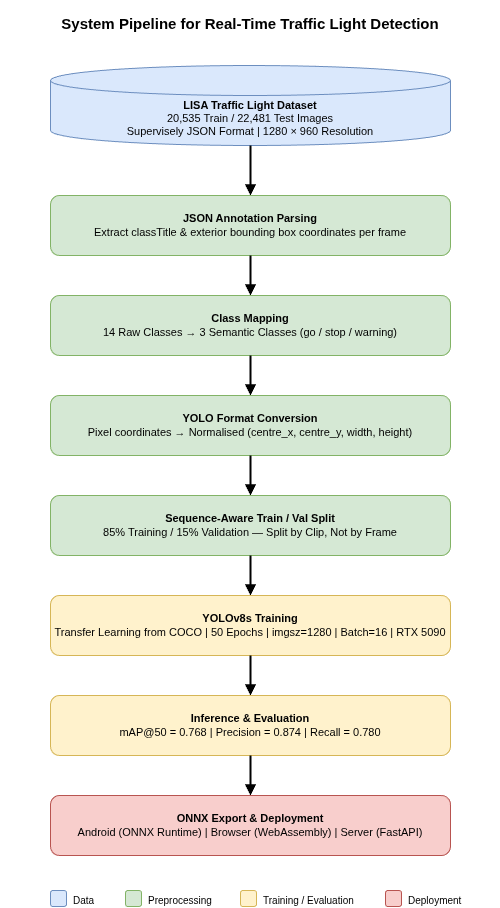
\includegraphics[width=0.92\textwidth,height=0.70\textheight,keepaspectratio]{Images/Diagrams/pipeline.png}
    \end{center}
    \caption{Overall system pipeline for traffic light detection.}
    \label{fig:pipeline}
\end{figure}

\section{Report Organisation}

The remainder of this report is organised as follows. Chapter~2 describes the LISA Traffic Light Dataset in detail, covering the annotation format, exploratory data analysis, class mapping, label conversion, data partitioning strategy, and class imbalance correction. Chapter~3 presents the YOLOv8s model architecture, the rationale for model selection, the transfer learning configuration, and an analysis of the training process including loss curves and accuracy progression. Chapter~4 presents the quantitative and qualitative evaluation results on both the validation and test sets, including per-class metrics, confusion matrix analysis, and sample inference visualisations. Chapter~5 summarises the achievements of the project, discusses the identified limitations, proposes directions for future work, and describes the available deployment pathways for the trained model.

%%%%%%%%%%%%%%%%%%%%%%%%%%%%%%%%%%%%%%%%%%%%%%%%%%%%%%%%%%%%%%%%%%%%%%%%%%%%%%%%%%%%%%%%%%%%%%%%%%
%%% END OF FILE
%%%%%%%%%%%%%%%%%%%%%%%%%%%%%%%%%%%%%%%%%%%%%%%%%%%%%%%%%%%%%%%%%%%%%%%%%%%%%%%%%%%%%%%%%%%%%%%%%%
